\documentclass{beamer}

% Should be documentclass beamer

\mode<presentation>
{
%  \usetheme[hideothersubsections]{PaloAlto}
  \usetheme{metropolis}
  \setbeamercovered{transparent}
}

\input{commonm}

\newcommand{\hdr}[2]{
  \title[CS 5220, Fall 2017]{CS 5220: #2}
  \author{David Bindel}
  \institute{Cornell}
  \date{#1}
}


\newcommand{\bfx}{\mathbf{x}}
\newcommand{\bfr}{\mathbf{r}}
\newcommand{\bfn}{\mathbf{n}}
\newcommand{\bfI}{\mathbf{I}}

\hdr{2017-11-07}{Graph Partitioning}

\begin{document}

% Graph partitioning task + terminology
% Applications
% Coordinate-based:
%   Coordinate bisection
%   Inertial partitioning
%   Circle partitioning (beyond hyperplanes) a la Gilbert
%     = centerpoint + random great circle
% Coordinate-free:
%   BFS / recursive graph bisection
%   Kernighan-Lin
%   Spectral partitioning
% Multilevel ideas
% Software

\begin{frame}
  \titlepage
\end{frame}


\begin{frame}
  \frametitle{Reminder: Sparsity and partitioning}

  \begin{center}
    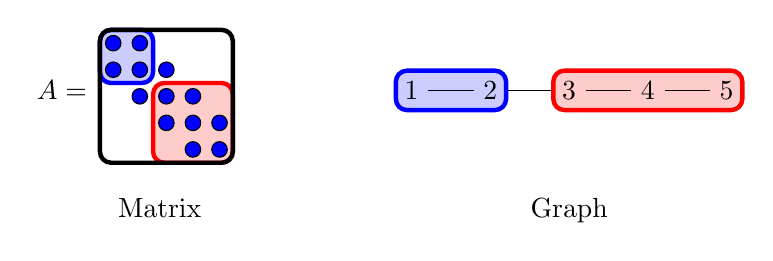
\begin{tikzpicture}

      % A = spy plot
      \draw (0,0.75) node[anchor=east] {$A=$};
      \begin{scope}[xshift=6pt,scale=2]
        \draw[ultra thick,rounded corners,color=blue,fill=blue!20] (-2.40pt,12.00pt) rectangle
        (7.20pt,21.60pt);
        \draw[ultra thick,rounded corners,color=red,fill=red!20] (7.20pt,12.00pt) rectangle
        (21.60pt,-2.40pt);

        \draw[ultra thick,rounded corners] (-2.40pt,21.60pt) rectangle (21.60pt,-2.40pt);
\draw[fill=blue] (0.00pt,19.20pt) circle [radius=1.4pt]; 
\draw[fill=blue] (4.80pt,19.20pt) circle [radius=1.4pt]; 
\draw[fill=blue] (0.00pt,14.40pt) circle [radius=1.4pt]; 
\draw[fill=blue] (4.80pt,14.40pt) circle [radius=1.4pt]; 
\draw[fill=blue] (9.60pt,14.40pt) circle [radius=1.4pt]; 
\draw[fill=blue] (4.80pt,9.60pt) circle [radius=1.4pt]; 
\draw[fill=blue] (9.60pt,9.60pt) circle [radius=1.4pt]; 
\draw[fill=blue] (14.40pt,9.60pt) circle [radius=1.4pt]; 
\draw[fill=blue] (9.60pt,4.80pt) circle [radius=1.4pt]; 
\draw[fill=blue] (14.40pt,4.80pt) circle [radius=1.4pt]; 
\draw[fill=blue] (19.20pt,4.80pt) circle [radius=1.4pt]; 
\draw[fill=blue] (14.40pt,0.00pt) circle [radius=1.4pt]; 
\draw[fill=blue] (19.20pt,0.00pt) circle [radius=1.4pt]; 

      \end{scope}

      % Graph picture
      \begin{scope}[xshift=4cm]
        \draw[ultra thick,rounded corners,color=blue,fill=blue!20]
          (-0.2,0.5) rectangle (1.2,1);
        \draw[ultra thick,rounded corners,color=red,fill=red!20]
          (1.8,0.5) rectangle (4.2,1);
        \node (A) at (0,0.75) {1};
        \node (B) at (1,0.75) {2};
        \node (C) at (2,0.75) {3};
        \node (D) at (3,0.75) {4};
        \node (E) at (4,0.75) {5};
        \draw (A) -- (B) -- (C) -- (D) -- (E);
      \end{scope}

      \node[anchor=north] at (0.8,-0.5) {Matrix};
      \node[anchor=north] at (6,-0.5) {Graph};
    \end{tikzpicture}
  \end{center}

  Want to partition sparse graphs so that
  \begin{itemize}
  \item Subgraphs are same size (load balance)
  \item Cut size is minimal (minimize communication)
  \end{itemize}
  Uses: parallel sparse matvec, nested dissection solves, ...

\end{frame}


\begin{frame}
  \frametitle{A common theme}

  Common idea: partition static data (or networked things):
  \begin{itemize}
  \item Physical network design (telephone layout, VLSI layout)
  \item Sparse matvec
  \item Preconditioners for PDE solvers
  \item Sparse Gaussian elimination
  \item Data clustering
  \item Image segmentation
  \end{itemize}
  Goal: Keep chunks big, minimize the ``surface area'' between
\end{frame}


\begin{frame}
  \frametitle{Graph partitioning}

  \begin{center}
    \begin{tikzpicture}[scale=0.7]
      \input{figs/part_ref.tikz}
    \end{tikzpicture}
  \end{center}
  
  Given: $G = (V,E)$, possibly with weights and coordinates. \\
  We want to partition $G$ into $k$ pieces such that
  \begin{itemize}
  \item
    Node weights are balanced across partitions.
  \item
    Weight of cut edges is minimized.
  \end{itemize}
  Important special case: $k = 2$.

\end{frame}


\begin{frame}
  \frametitle{Graph partitioning: Vertex separator}

  \begin{center}
    \begin{tikzpicture}
      \input{figs/part_vsep.tikz}
    \end{tikzpicture}
  \end{center}
\end{frame}


\begin{frame}
  \frametitle{Graph partitioning: Edge separator}

  \begin{center}
    \begin{tikzpicture}
      \input{figs/part_esep.tikz}
    \end{tikzpicture}
  \end{center}
\end{frame}


\begin{frame}
  \frametitle{Node to edge and back again}

  \begin{tikzpicture}[scale=0.7]
    \begin{scope}
      \input{figs/part_vsep.tikz}
    \end{scope}

    \draw[ultra thick,<->] (5,1) -- (7,1);
    
    \begin{scope}[xshift=8cm]
      \input{figs/part_esep.tikz}
    \end{scope}
  \end{tikzpicture}

  \vspace{3mm}
  Can convert between node and edge separators
  \begin{itemize}
  \item Node to edge: cut all edges from separator to one side
  \item Edge to node: remove nodes on one side of cut edges
  \end{itemize}
  Fine if graph is degree bounded (e.g.~near-neighbor meshes). \\
  Optimal vertex/edge separators very different for social networks!
  
\end{frame}


\begin{frame}
  \frametitle{Cost}

  How many partitionings are there?  If $n$ is even,
  \[
    \begin{pmatrix} n \\ n/2 \end{pmatrix} =
    \frac{n!}{( (n/2)! )^2} \approx 
    2^n \sqrt{2/(\pi n)}.
  \]
  Finding the optimal one is NP-complete.

  \vspace{1cm}
  We need heuristics!
\end{frame}


\begin{frame}
  \frametitle{Partitioning with coordinates}

  \begin{itemize}
  \item Lots of partitioning problems from ``nice'' meshes
    \begin{itemize}
    \item Planar meshes (maybe with regularity condition)
    \item $k$-ply meshes (works for $d > 2$)
    \item Nice enough $\implies$ partition with $O(n^{1-1/d})$ edge cuts \\
      (Tarjan, Lipton; Miller, Teng, Thurston, Vavasis)
    \item Edges link nearby vertices
    \end{itemize}
  \item Get useful information from vertex density
  \item Ignore edges (but can use them in later refinement)
  \end{itemize}
  
\end{frame}


\begin{frame}
  \frametitle{Recursive coordinate bisection}

  \begin{center}
    \begin{tikzpicture}[scale=0.7]
      \input{figs/part_esep_bisect.tikz}
    \end{tikzpicture}
  \end{center}
  
  Idea: Cut with hyperplane parallel to a coordinate axis.
  \begin{itemize}
  \item Pro: Fast and simple
  \item Con: Not always great quality
  \end{itemize}
\end{frame}


\begin{frame}
  \frametitle{Inertial bisection}

  Idea: Optimize cutting hyperplane based on vertex density
  \begin{align*}
    \bar{\bfx} &= \frac{1}{n} \sum_{i=1}^n \bfx_i \\
    \bar{\bfr_i} &= \bfx_i-\bar{\bfx} \\
    \bfI &= \sum_{i=1}^n\left[ \|\bfr_i\|^2 I - \bfr_i \bfr_i^T \right]
  \end{align*}
  Let $(\lambda_n, \bfn)$ be the minimal eigenpair for the inertia
  tensor $\bfI$, and choose the hyperplane through $\bar{\bfx}$ 
  with normal $\bfn$.  
  
\end{frame}


\begin{frame}
  \frametitle{Inertial bisection}

  \begin{center}
    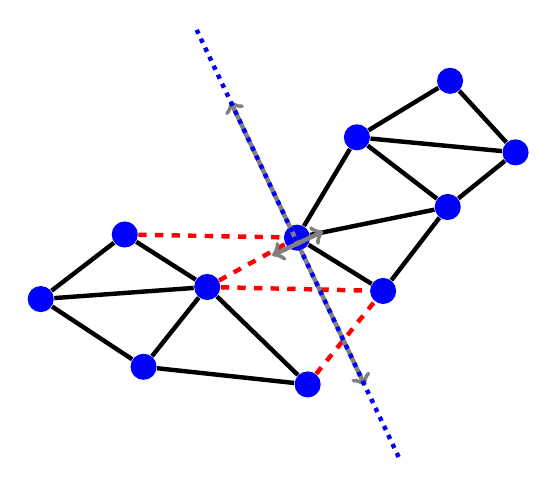
\begin{tikzpicture}
      \node (n1) at (1.108060,0.168294) [circle,fill=blue] {};
\node (n2) at (1.916771,1.181859) [circle,fill=blue] {};
\node (n3) at (-0.197998,1.028224) [circle,fill=blue] {};
\node (n4) at (0.869271,1.848640) [circle,fill=blue] {};
\node (n5) at (3.056732,1.808215) [circle,fill=blue] {};
\node (n6) at (3.192034,-0.055883) [circle,fill=blue] {};
\node (n7) at (4.150780,1.131397) [circle,fill=blue] {};
\node (n8) at (4.970900,2.197872) [circle,fill=blue] {};
\node (n9) at (3.817774,3.082424) [circle,fill=blue] {};
\node (n10) at (5.832186,2.891196) [circle,fill=blue] {};
\node (n11) at (5.000885,3.800002) [circle,fill=blue] {};
\draw[    ultra thick       ] (n1) -- (n2);
\draw[    ultra thick       ] (n1) -- (n3);
\draw[    ultra thick       ] (n1) -- (n6);
\draw[    ultra thick       ] (n2) -- (n3);
\draw[    ultra thick       ] (n2) -- (n4);
\draw[red,ultra thick,dashed] (n2) -- (n5);
\draw[    ultra thick       ] (n2) -- (n6);
\draw[red,ultra thick,dashed] (n2) -- (n7);
\draw[    ultra thick       ] (n3) -- (n4);
\draw[red,ultra thick,dashed] (n4) -- (n5);
\draw[    ultra thick       ] (n5) -- (n7);
\draw[    ultra thick       ] (n5) -- (n8);
\draw[    ultra thick       ] (n5) -- (n9);
\draw[red,ultra thick,dashed] (n6) -- (n7);
\draw[    ultra thick       ] (n7) -- (n8);
\draw[    ultra thick       ] (n8) -- (n9);
\draw[    ultra thick       ] (n8) -- (n10);
\draw[    ultra thick       ] (n9) -- (n10);
\draw[    ultra thick       ] (n9) -- (n11);
\draw[    ultra thick       ] (n10) -- (n11);
\draw[black!50,ultra thick,<->] (3.388714,1.887715) -- (2.741721,1.581784);
\draw[black!50,ultra thick,<->] (3.920159,-0.073310) -- (2.210277,3.542808);
\draw[blue, ultra thick,dotted] (4.347629,-0.977339) -- (1.782806,4.446837);

    \end{tikzpicture}
  \end{center}

  \begin{itemize}
  \item Pro: Still simple, more flexible than coordinate planes
  \item Con: Still restricted to hyperplanes
  \end{itemize}
\end{frame}



\begin{frame}
  \frametitle{Random circles (Gilbert, Miller, Teng)}
  
  \begin{itemize}
  \item Stereographic projection
  \item Find centerpoint (any plane is an even partition) \\
    In practice, use an approximation.
  \item Conformally map sphere, moving centerpoint to origin
  \item Choose great circle (at random)
  \item Undo stereographic projection
  \item Convert circle to separator
  \end{itemize}
  May choose best of several random great circles.
\end{frame}


\begin{frame}
  \frametitle{Coordinate-free methods}

  \begin{center}
    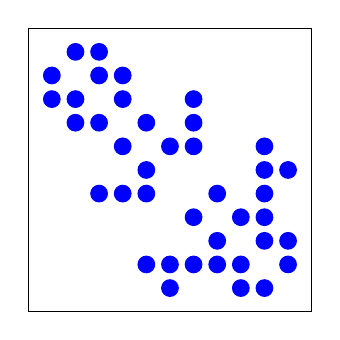
\begin{tikzpicture}
      \draw (-0.3,0) rectangle (3.300000,3.600000);
\filldraw[blue] (3.000000,0.600000) circle (3pt);
\filldraw[blue] (3.000000,0.900000) circle (3pt);
\filldraw[blue] (3.000000,1.800000) circle (3pt);
\filldraw[blue] (2.700000,0.300000) circle (3pt);
\filldraw[blue] (2.700000,0.900000) circle (3pt);
\filldraw[blue] (2.700000,1.200000) circle (3pt);
\filldraw[blue] (2.700000,1.500000) circle (3pt);
\filldraw[blue] (2.700000,1.800000) circle (3pt);
\filldraw[blue] (2.700000,2.100000) circle (3pt);
\filldraw[blue] (2.400000,0.300000) circle (3pt);
\filldraw[blue] (2.400000,0.600000) circle (3pt);
\filldraw[blue] (2.400000,1.200000) circle (3pt);
\filldraw[blue] (2.100000,0.600000) circle (3pt);
\filldraw[blue] (2.100000,0.900000) circle (3pt);
\filldraw[blue] (2.100000,1.500000) circle (3pt);
\filldraw[blue] (1.800000,0.600000) circle (3pt);
\filldraw[blue] (1.800000,1.200000) circle (3pt);
\filldraw[blue] (1.800000,2.100000) circle (3pt);
\filldraw[blue] (1.800000,2.400000) circle (3pt);
\filldraw[blue] (1.800000,2.700000) circle (3pt);
\filldraw[blue] (1.500000,0.300000) circle (3pt);
\filldraw[blue] (1.500000,0.600000) circle (3pt);
\filldraw[blue] (1.500000,2.100000) circle (3pt);
\filldraw[blue] (1.200000,0.600000) circle (3pt);
\filldraw[blue] (1.200000,1.500000) circle (3pt);
\filldraw[blue] (1.200000,1.800000) circle (3pt);
\filldraw[blue] (1.200000,2.400000) circle (3pt);
\filldraw[blue] (0.900000,1.500000) circle (3pt);
\filldraw[blue] (0.900000,2.100000) circle (3pt);
\filldraw[blue] (0.900000,2.700000) circle (3pt);
\filldraw[blue] (0.900000,3.000000) circle (3pt);
\filldraw[blue] (0.600000,1.500000) circle (3pt);
\filldraw[blue] (0.600000,2.400000) circle (3pt);
\filldraw[blue] (0.600000,3.000000) circle (3pt);
\filldraw[blue] (0.600000,3.300000) circle (3pt);
\filldraw[blue] (0.300000,2.400000) circle (3pt);
\filldraw[blue] (0.300000,2.700000) circle (3pt);
\filldraw[blue] (0.300000,3.300000) circle (3pt);
\filldraw[blue] (0.000000,2.700000) circle (3pt);
\filldraw[blue] (0.000000,3.000000) circle (3pt);

    \end{tikzpicture}
  \end{center}
  
  \begin{itemize}
  \item Don't always have natural coordinates
    \begin{itemize}
    \item Example: the web graph
    \item Can sometimes add coordinates (metric embedding)
    \end{itemize}
  \item So use edge information for geometry!
  \end{itemize}
\end{frame}


\begin{frame}
  \frametitle{Breadth-first search}

  \begin{center}
    \begin{tikzpicture}[scale=0.7]
      \input{figs/part_bfs.tikz}
    \end{tikzpicture}
  \end{center}
  
  \begin{itemize}
  \item Pick a start vertex $v_0$
    \begin{itemize}
    \item Might start from several different vertices
    \end{itemize}
  \item Use BFS to label nodes by distance from $v_0$
    \begin{itemize}
    \item We've seen this before -- remember RCM?
    \item Could use a different order -- minimize edge cuts locally \\
      (Karypis, Kumar)
    \end{itemize}
  \item Partition by distance from $v_0$
  \end{itemize}
\end{frame}


\begin{frame}
  \frametitle{Spectral partitioning}

  Label vertex $i$ with $x_i = \pm 1$.  We want to minimize
  \[
    \mbox{edges cut} = \frac{1}{4} \sum_{(i,j) \in E} (x_i-x_j)^2
  \]
  subject to the even partition requirement
  \[
    \sum_i x_i = 0.
  \]
  But this is NP hard, so we need a trick.

\end{frame}


\begin{frame}
  \frametitle{Spectral partitioning}

  Write
  \[
    \mbox{edges cut} 
    = \frac{1}{4} \sum_{(i,j) \in E} (x_i-x_j)^2 
    = \frac{1}{4} \|Cx\|^2 = \frac{1}{4} x^T L x
  \]
  where $C$ is the incidence matrix and $L = C^T C$ is the graph Laplacian:
  \begin{align*}
    C_{ij} &= 
      \begin{cases}
         1, & e_j = (i,k) \\
        -1, & e_j = (k,i) \\
         0, & \mbox{otherwise},
      \end{cases} &
    L_{ij} &= 
    \begin{cases} 
      d(i), & i = j \\
      -1, & i \neq j, (i,j) \in E, \\ 
      0, & \mbox{otherwise}.
    \end{cases}
  \end{align*}
  Note that $C e = 0$ (so $L e = 0$), $e = (1, 1, 1, \ldots, 1)^T$.

\end{frame}


\begin{frame}
  \frametitle{Spectral partitioning}

  Now consider the {\em relaxed} problem with $x \in \bbR^n$:
  \[
    \mbox{minimize } x^T L x \mbox{ s.t. } x^T e = 0 \mbox{ and } x^T x = 1.
  \]
  Equivalent to finding the second-smallest eigenvalue $\lambda_2$
  and corresponding eigenvector $x$, also called the {\em Fiedler vector}.
  Partition according to sign of $x_i$.

  \vspace{5mm}
  How to approximate $x$?  Use a Krylov subspace method (Lanczos)!
  Expensive, but gives high-quality partitions.
\end{frame}


\begin{frame}
  \frametitle{Spectral partitioning}

  \begin{center}
    \begin{tikzpicture}
      \input{figs/part_esep_spectral.tikz}
    \end{tikzpicture}
  \end{center}
\end{frame}


\begin{frame}
  \frametitle{Spectral coordinates}

  \begin{center}
    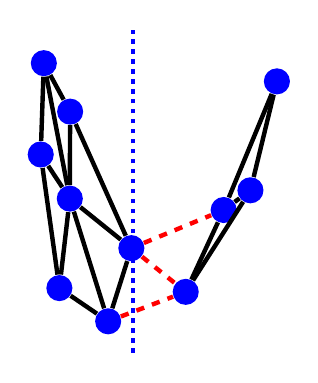
\begin{tikzpicture}[scale=0.7]
      \node (n1) at (-1.669431,0.758013) [circle,fill=blue] {};
\node (n2) at (-1.141880,-0.042414) [circle,fill=blue] {};
\node (n3) at (-1.612893,2.414905) [circle,fill=blue] {};
\node (n4) at (-1.135961,1.535636) [circle,fill=blue] {};
\node (n5) at (-0.025292,-0.940933) [circle,fill=blue] {};
\node (n6) at (-1.330865,-1.665852) [circle,fill=blue] {};
\node (n7) at (-0.445748,-2.268549) [circle,fill=blue] {};
\node (n8) at (0.961399,-1.734149) [circle,fill=blue] {};
\node (n9) at (1.649706,-0.249551) [circle,fill=blue] {};
\node (n10) at (2.135590,0.108266) [circle,fill=blue] {};
\node (n11) at (2.615375,2.084628) [circle,fill=blue] {};
\draw[    ultra thick       ] (n1) -- (n2);
\draw[    ultra thick       ] (n1) -- (n3);
\draw[    ultra thick       ] (n1) -- (n6);
\draw[    ultra thick       ] (n2) -- (n3);
\draw[    ultra thick       ] (n2) -- (n4);
\draw[    ultra thick       ] (n2) -- (n5);
\draw[    ultra thick       ] (n2) -- (n6);
\draw[    ultra thick       ] (n2) -- (n7);
\draw[    ultra thick       ] (n3) -- (n4);
\draw[    ultra thick       ] (n4) -- (n5);
\draw[    ultra thick       ] (n5) -- (n7);
\draw[red,ultra thick,dashed] (n5) -- (n8);
\draw[red,ultra thick,dashed] (n5) -- (n9);
\draw[    ultra thick       ] (n6) -- (n7);
\draw[red,ultra thick,dashed] (n7) -- (n8);
\draw[    ultra thick       ] (n8) -- (n9);
\draw[    ultra thick       ] (n8) -- (n10);
\draw[    ultra thick       ] (n9) -- (n10);
\draw[    ultra thick       ] (n9) -- (n11);
\draw[    ultra thick       ] (n10) -- (n11);
\draw[blue, ultra thick,dotted] (0,-2.835686) -- (0,3.018631);

    \end{tikzpicture}
  \end{center}
  
  Alternate view: define a coordinate system with the first $d$
  non-trivial Laplacian eigenvectors.
  \begin{itemize}
  \item Spectral partitioning = bisection in spectral coordinates
  \item Can cluster in other ways as well (e.g. $k$-means)
  \end{itemize}
  
\end{frame}


\begin{frame}
  \frametitle{Refinement by swapping}

  \begin{center}
    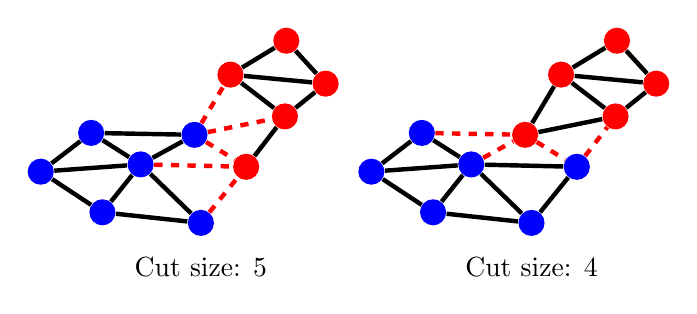
\begin{tikzpicture}[scale=0.6]
      \begin{scope}[xshift=0.000000cm]
\node (n1) at (1.108060,0.168294) [circle,fill=blue] {};
\node (n2) at (1.916771,1.181859) [circle,fill=blue] {};
\node (n3) at (-0.197998,1.028224) [circle,fill=blue] {};
\node (n4) at (0.869271,1.848640) [circle,fill=blue] {};
\node (n5) at (3.056732,1.808215) [circle,fill=blue] {};
\node (n6) at (3.192034,-0.055883) [circle,fill=blue] {};
\node (n7) at (4.150780,1.131397) [circle,fill=red] {};
\node (n8) at (4.970900,2.197872) [circle,fill=red] {};
\node (n9) at (3.817774,3.082424) [circle,fill=red] {};
\node (n10) at (5.832186,2.891196) [circle,fill=red] {};
\node (n11) at (5.000885,3.800002) [circle,fill=red] {};
\draw[    ultra thick       ] (n1) -- (n2);
\draw[    ultra thick       ] (n1) -- (n3);
\draw[    ultra thick       ] (n1) -- (n6);
\draw[    ultra thick       ] (n2) -- (n3);
\draw[    ultra thick       ] (n2) -- (n4);
\draw[    ultra thick       ] (n2) -- (n5);
\draw[    ultra thick       ] (n2) -- (n6);
\draw[red,ultra thick,dashed] (n2) -- (n7);
\draw[    ultra thick       ] (n3) -- (n4);
\draw[    ultra thick       ] (n4) -- (n5);
\draw[red,ultra thick,dashed] (n5) -- (n7);
\draw[red,ultra thick,dashed] (n5) -- (n8);
\draw[red,ultra thick,dashed] (n5) -- (n9);
\draw[red,ultra thick,dashed] (n6) -- (n7);
\draw[    ultra thick       ] (n7) -- (n8);
\draw[    ultra thick       ] (n8) -- (n9);
\draw[    ultra thick       ] (n8) -- (n10);
\draw[    ultra thick       ] (n9) -- (n10);
\draw[    ultra thick       ] (n9) -- (n11);
\draw[    ultra thick       ] (n10) -- (n11);
\node at (3.192034,-1) {Cut size: 5};
\end{scope}
\begin{scope}[xshift=6.998623cm]
\node (n1) at (1.108060,0.168294) [circle,fill=blue] {};
\node (n2) at (1.916771,1.181859) [circle,fill=blue] {};
\node (n3) at (-0.197998,1.028224) [circle,fill=blue] {};
\node (n4) at (0.869271,1.848640) [circle,fill=blue] {};
\node (n5) at (3.056732,1.808215) [circle,fill=red] {};
\node (n6) at (3.192034,-0.055883) [circle,fill=blue] {};
\node (n7) at (4.150780,1.131397) [circle,fill=blue] {};
\node (n8) at (4.970900,2.197872) [circle,fill=red] {};
\node (n9) at (3.817774,3.082424) [circle,fill=red] {};
\node (n10) at (5.832186,2.891196) [circle,fill=red] {};
\node (n11) at (5.000885,3.800002) [circle,fill=red] {};
\draw[    ultra thick       ] (n1) -- (n2);
\draw[    ultra thick       ] (n1) -- (n3);
\draw[    ultra thick       ] (n1) -- (n6);
\draw[    ultra thick       ] (n2) -- (n3);
\draw[    ultra thick       ] (n2) -- (n4);
\draw[red,ultra thick,dashed] (n2) -- (n5);
\draw[    ultra thick       ] (n2) -- (n6);
\draw[    ultra thick       ] (n2) -- (n7);
\draw[    ultra thick       ] (n3) -- (n4);
\draw[red,ultra thick,dashed] (n4) -- (n5);
\draw[red,ultra thick,dashed] (n5) -- (n7);
\draw[    ultra thick       ] (n5) -- (n8);
\draw[    ultra thick       ] (n5) -- (n9);
\draw[    ultra thick       ] (n6) -- (n7);
\draw[red,ultra thick,dashed] (n7) -- (n8);
\draw[    ultra thick       ] (n8) -- (n9);
\draw[    ultra thick       ] (n8) -- (n10);
\draw[    ultra thick       ] (n9) -- (n10);
\draw[    ultra thick       ] (n9) -- (n11);
\draw[    ultra thick       ] (n10) -- (n11);
\node at (3.192034,-1) {Cut size: 4};
\end{scope}

    \end{tikzpicture}
  \end{center}
  Gain from swapping $(a,b)$ is $D(a) + D(b) - 2w(a,b)$, where \\
  $D$ is external - internal edge costs:
  \begin{align*}
    D(a) &= \sum_{b' \in B} w(a,b') - \sum_{a' \in A, a' \neq a} w(a,a') \\
    D(b) &= \sum_{a' \in A} w(b,a') - \sum_{b' \in B, b' \neq b} w(b,b') 
  \end{align*}
\end{frame}


\begin{frame}
  \frametitle{Greedy refinement}

  \begin{center}
    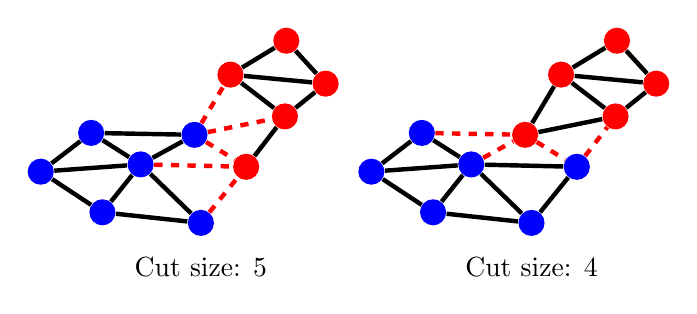
\begin{tikzpicture}[scale=0.6]
      \begin{scope}[xshift=0.000000cm]
\node (n1) at (1.108060,0.168294) [circle,fill=blue] {};
\node (n2) at (1.916771,1.181859) [circle,fill=blue] {};
\node (n3) at (-0.197998,1.028224) [circle,fill=blue] {};
\node (n4) at (0.869271,1.848640) [circle,fill=blue] {};
\node (n5) at (3.056732,1.808215) [circle,fill=blue] {};
\node (n6) at (3.192034,-0.055883) [circle,fill=blue] {};
\node (n7) at (4.150780,1.131397) [circle,fill=red] {};
\node (n8) at (4.970900,2.197872) [circle,fill=red] {};
\node (n9) at (3.817774,3.082424) [circle,fill=red] {};
\node (n10) at (5.832186,2.891196) [circle,fill=red] {};
\node (n11) at (5.000885,3.800002) [circle,fill=red] {};
\draw[    ultra thick       ] (n1) -- (n2);
\draw[    ultra thick       ] (n1) -- (n3);
\draw[    ultra thick       ] (n1) -- (n6);
\draw[    ultra thick       ] (n2) -- (n3);
\draw[    ultra thick       ] (n2) -- (n4);
\draw[    ultra thick       ] (n2) -- (n5);
\draw[    ultra thick       ] (n2) -- (n6);
\draw[red,ultra thick,dashed] (n2) -- (n7);
\draw[    ultra thick       ] (n3) -- (n4);
\draw[    ultra thick       ] (n4) -- (n5);
\draw[red,ultra thick,dashed] (n5) -- (n7);
\draw[red,ultra thick,dashed] (n5) -- (n8);
\draw[red,ultra thick,dashed] (n5) -- (n9);
\draw[red,ultra thick,dashed] (n6) -- (n7);
\draw[    ultra thick       ] (n7) -- (n8);
\draw[    ultra thick       ] (n8) -- (n9);
\draw[    ultra thick       ] (n8) -- (n10);
\draw[    ultra thick       ] (n9) -- (n10);
\draw[    ultra thick       ] (n9) -- (n11);
\draw[    ultra thick       ] (n10) -- (n11);
\node at (3.192034,-1) {Cut size: 5};
\end{scope}
\begin{scope}[xshift=6.998623cm]
\node (n1) at (1.108060,0.168294) [circle,fill=blue] {};
\node (n2) at (1.916771,1.181859) [circle,fill=blue] {};
\node (n3) at (-0.197998,1.028224) [circle,fill=blue] {};
\node (n4) at (0.869271,1.848640) [circle,fill=blue] {};
\node (n5) at (3.056732,1.808215) [circle,fill=red] {};
\node (n6) at (3.192034,-0.055883) [circle,fill=blue] {};
\node (n7) at (4.150780,1.131397) [circle,fill=blue] {};
\node (n8) at (4.970900,2.197872) [circle,fill=red] {};
\node (n9) at (3.817774,3.082424) [circle,fill=red] {};
\node (n10) at (5.832186,2.891196) [circle,fill=red] {};
\node (n11) at (5.000885,3.800002) [circle,fill=red] {};
\draw[    ultra thick       ] (n1) -- (n2);
\draw[    ultra thick       ] (n1) -- (n3);
\draw[    ultra thick       ] (n1) -- (n6);
\draw[    ultra thick       ] (n2) -- (n3);
\draw[    ultra thick       ] (n2) -- (n4);
\draw[red,ultra thick,dashed] (n2) -- (n5);
\draw[    ultra thick       ] (n2) -- (n6);
\draw[    ultra thick       ] (n2) -- (n7);
\draw[    ultra thick       ] (n3) -- (n4);
\draw[red,ultra thick,dashed] (n4) -- (n5);
\draw[red,ultra thick,dashed] (n5) -- (n7);
\draw[    ultra thick       ] (n5) -- (n8);
\draw[    ultra thick       ] (n5) -- (n9);
\draw[    ultra thick       ] (n6) -- (n7);
\draw[red,ultra thick,dashed] (n7) -- (n8);
\draw[    ultra thick       ] (n8) -- (n9);
\draw[    ultra thick       ] (n8) -- (n10);
\draw[    ultra thick       ] (n9) -- (n10);
\draw[    ultra thick       ] (n9) -- (n11);
\draw[    ultra thick       ] (n10) -- (n11);
\node at (3.192034,-1) {Cut size: 4};
\end{scope}

    \end{tikzpicture}
  \end{center}
  Start with a partition $V = A \cup B$ and refine.
  \begin{itemize}
  \item $\operatorname{gain}(a,b) = D(a) + D(b) - 2w(a,b)$
  \item Purely greedy strategy: until no positive gain
    \begin{itemize}
    \item Choose swap with most gain
    \item Update $D$ in neighborhood of swap; update gains
    \end{itemize}
  \item Local minima are a problem.
  \end{itemize}
\end{frame}


\begin{frame}
  \frametitle{Kernighan-Lin}

  In one sweep:
  \begin{tabbing}
    \qquad \= \kill
    While no vertices marked \\
    \> Choose $(a,b)$ with greatest gain \\
    \> Update $D(v)$ for all unmarked $v$ as if $(a,b)$ were swapped \\
    \> Mark $a$ and $b$ (but don't swap) \\
    Find $j$ such that swaps $1, \ldots, j$ yield maximal gain \\
    Apply swaps $1, \ldots, j$
  \end{tabbing}
  Usually converges in a few (2-6) sweeps.  Each sweep is $O(|V|^3)$.
  Can be improved to $O(|E|)$ (Fiduccia, Mattheyses).
  
  \vspace{5mm}
  Further improvements (Karypis, Kumar): only consider vertices on boundary,
  don't complete full sweep.
\end{frame}


\begin{frame}
  \frametitle{Multilevel ideas}

  Basic idea (same will work in other contexts):
  \begin{itemize}
  \item Coarsen
  \item Solve coarse problem
  \item Interpolate (and possibly refine)
  \end{itemize}
  May apply recursively.

\end{frame}


\begin{frame}
  \frametitle{Maximal matching}

  One idea for coarsening: maximal matchings
  \begin{itemize}
  \item
    {\em Matching} of $G = (V,E)$ is $E_m \subset E$ with no common vertices.
  \item
    {\em Maximal}: cannot add edges and remain matching.
  \item
    Constructed by an obvious greedy algorithm.
  \item
    Maximal matchings are non-unique; some may be preferable to others
    (e.g. choose heavy edges first).
  \end{itemize}
\end{frame}


\begin{frame}
  \frametitle{Coarsening via maximal matching}

  \begin{center}
    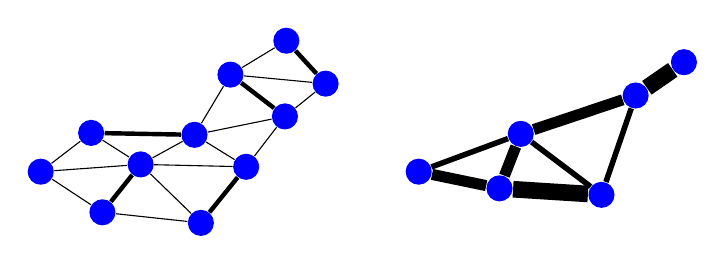
\begin{tikzpicture}[scale=0.6]
      \begin{scope}
        \node (n1) at (1.108060,0.168294) [circle,fill=blue] {};
\node (n2) at (1.916771,1.181859) [circle,fill=blue] {};
\node (n3) at (-0.197998,1.028224) [circle,fill=blue] {};
\node (n4) at (0.869271,1.848640) [circle,fill=blue] {};
\node (n5) at (3.056732,1.808215) [circle,fill=blue] {};
\node (n6) at (3.192034,-0.055883) [circle,fill=blue] {};
\node (n7) at (4.150780,1.131397) [circle,fill=blue] {};
\node (n8) at (4.970900,2.197872) [circle,fill=blue] {};
\node (n9) at (3.817774,3.082424) [circle,fill=blue] {};
\node (n10) at (5.832186,2.891196) [circle,fill=blue] {};
\node (n11) at (5.000885,3.800002) [circle,fill=blue] {};
\draw (n1) -- (n2);
\draw (n1) -- (n3);
\draw (n1) -- (n6);
\draw (n2) -- (n3);
\draw (n2) -- (n4);
\draw (n2) -- (n5);
\draw (n2) -- (n6);
\draw (n2) -- (n7);
\draw (n3) -- (n4);
\draw (n4) -- (n5);
\draw (n5) -- (n7);
\draw (n5) -- (n8);
\draw (n5) -- (n9);
\draw (n6) -- (n7);
\draw (n7) -- (n8);
\draw (n8) -- (n9);
\draw (n8) -- (n10);
\draw (n9) -- (n10);
\draw (n9) -- (n11);
\draw (n10) -- (n11);
\draw[ultra thick] (n1) -- (n2);
\draw[ultra thick] (n3) -- (n3);
\draw[ultra thick] (n4) -- (n5);
\draw[ultra thick] (n6) -- (n7);
\draw[ultra thick] (n8) -- (n9);
\draw[ultra thick] (n10) -- (n11);

      \end{scope}
      \begin{scope}[xshift=8cm]
        \node (n1) at (1.512416,0.675077) [circle,fill=blue] {};
\node (n2) at (-0.197998,1.028224) [circle,fill=blue] {};
\node (n3) at (1.963002,1.828427) [circle,fill=blue] {};
\node (n4) at (3.671407,0.537757) [circle,fill=blue] {};
\node (n5) at (4.394337,2.640148) [circle,fill=blue] {};
\node (n6) at (5.416535,3.345599) [circle,fill=blue] {};
\draw[line width=4pt] (n1) -- (n1);
\draw[line width=4pt] (n1) -- (n2);
\draw[line width=4pt] (n1) -- (n3);
\draw[line width=2pt] (n2) -- (n3);
\draw[line width=4pt] (n3) -- (n3);
\draw[line width=6pt] (n1) -- (n4);
\draw[line width=2pt] (n3) -- (n4);
\draw[line width=4pt] (n4) -- (n4);
\draw[line width=4pt] (n3) -- (n5);
\draw[line width=2pt] (n4) -- (n5);
\draw[line width=4pt] (n5) -- (n5);
\draw[line width=6pt] (n5) -- (n6);
\draw[line width=4pt] (n6) -- (n6);

      \end{scope}
    \end{tikzpicture}
  \end{center}

  \begin{itemize}
  \item Collapse nodes connected in matching into coarse nodes
  \item Add all edge weights between connected coarse nodes
  \end{itemize}
\end{frame}


\begin{frame}
  \frametitle{Software}

  All these use some flavor(s) of multilevel:
  \begin{itemize}
  \item METIS/ParMETIS (Kapyris)
  \item PARTY (U. Paderborn)
  \item Chaco (Sandia)
  \item Scotch (INRIA)
  \item Jostle (now commercialized)
  \item Zoltan (Sandia)
  \end{itemize}
\end{frame}


\begin{frame}
  \frametitle{Graph partitioning: Is this it?}

  Consider partitioning just for sparse matvec:
  \begin{itemize}
  \item Edge cuts $\neq$ communication volume
  \item Should we minimize {\em max} communication volume?
  \item Looked at communication volume -- what about latencies?
  \end{itemize}
  Some go beyond graph partitioning (e.g.~hypergraph in Zoltan).
\end{frame}

\begin{frame}
  \frametitle{Graph partitioning: Is this it?}

  Additional work on:
  \begin{itemize}
  \item Partitioning power law graphs
  \item Covering sets with small overlaps
  \end{itemize}
  Also: Classes of graphs with no small cuts (expanders)

\end{frame}

\begin{frame}
  \frametitle{Graph partitioning: Is this it?}

  Recall: partitioning for matvec {\em and} preconditioner
  \begin{itemize}
  \item Block Jacobi (or Schwarz) -- relax on each partition
  \item Want to consider edge cuts {\em and physics}
    \begin{itemize}
    \item E.g.~consider edges = beams
    \item Cutting a stiff beam worse than a flexible beam?
    \item Doesn't show up from just the topology
    \end{itemize}
  \item Multiple ways to deal with this
    \begin{itemize}
    \item Encode physics via edge weights?
    \item Partition geometrically?
    \end{itemize}
  \item Tradeoffs are why we need to be {\em informed} users
  \end{itemize}
\end{frame}

\begin{frame}
  \frametitle{Graph partitioning: Is this it?}

  So far, considered problems with {\em static} interactions
  \begin{itemize}
  \item What about particle simulations?
  \item Or what about tree searches?
  \item Or what about...?
  \end{itemize}
  Next time: more general {\em load balancing} issues
\end{frame}

\end{document}
